\subsection{Web}
The primary focus lied within the application functionality, the design was made using Bootstrap\cite{ref_bootstrap}. 
The basic design of the site is a top navigation bar with a Menu dropdown containing tabs which makes the user be able to handle game, lobby and friend service options. A  ``Create Game'' menu which contains the options to either start 2 or 4 player lobbies where the user can invite friends to their lobby before starting a game with them. There's also the possibility to start the lobby before it's full. This will fill the rest of the lobby up with other players before the game is created. Alternatively there's an option to directly put the user into a 2 or 4 player queue by using the QuickJoin option for either game mode. There's also a Username and password field in the navbar along a Register Link to be able to register/login into the site.

\begin{figure}[H]
	\centering
	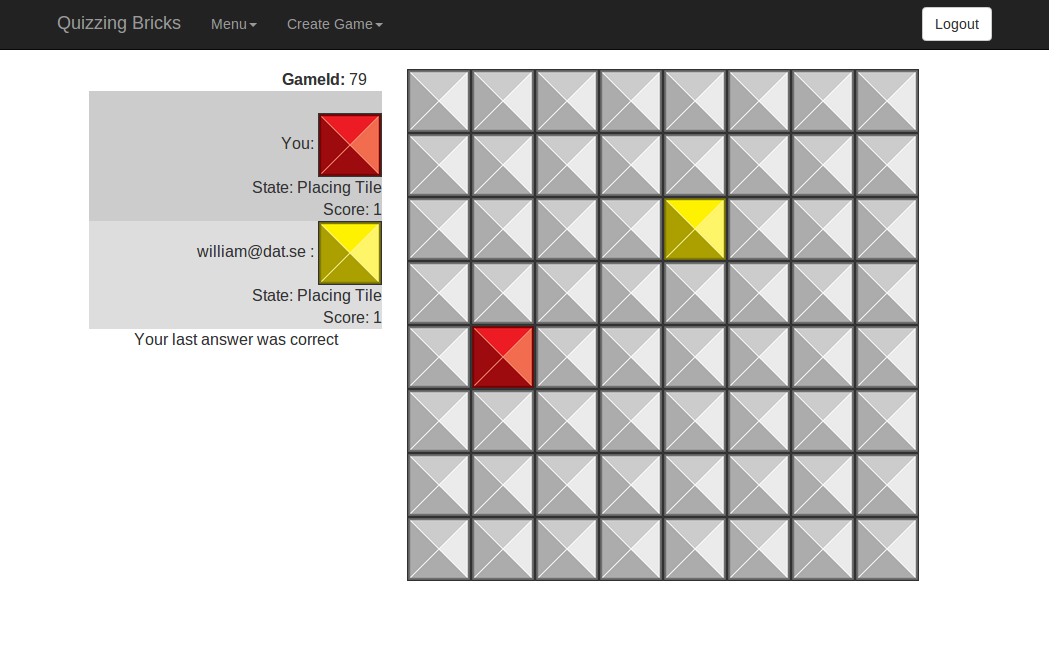
\includegraphics[width=\textwidth,height=\textheight,keepaspectratio=true]{img/game_board_page.png}
	\caption{The client website during a game.}
	\label{fig:web}
\end{figure}

As shown in Figure \ref{fig:web} the game board page basically contains a player status container on the left giving information about the color of the different players and their current game status (if they're placing tiles / answering question etc) and their current score in the game. On the Right side there's  a game board which is build with a grey base tile which is overwritten by the corresponding players tile when they have won that specific tile, this game board is of the size 8x8 in the current version but can easily be expanded by changing the loop variable for creating the board.

\subsection{Mobile Clients}
One focus in the design was that the applications should look and handle the same way. This was later determined to not be the best approach because of the differences between android and iOS design guidelines. The functionality in Android and iOS handles the same with some minor differences concerning the placement of where you can find and handle lobbies.\\
The only other major difference is, as mentioned before, the graphic design and what additional libraries we use for example communication. 

